\section{Single-Day Validation Results}
\label{sec:single_day}

Before extending to multi-day regimes, we establish that LLMs can detect single-day dealer constraints under obfuscation---a prerequisite for temporal regime identification. This section summarizes results from our companion single-day study \citep{regan2025obfuscation} and presents the raw chain validation that motivates the regime detection extension.

\subsection{Detection Under Obfuscation}

Applied to 242 trading days (SPY, 2024), the obfuscation framework achieved 71.5\% detection of dealer hedging patterns using unbiased prompts, with 90.9\% predictive accuracy on forward returns. The WHO$\rightarrow$WHOM$\rightarrow$WHAT causal framework achieved $>$90\% correct specification across all three components, confirming the model articulates mechanical reasoning rather than pattern labels.

Detection remained stable across quarters: 68.3\% (Q1), 74.2\% (Q2), 71.7\% (Q3), and 72.1\% (Q4), with no statistically significant seasonal variation ($p = 0.84$). This temporal stability is critical---it confirms the framework identifies structural properties rather than period-specific memorization.

\subsection{Raw Chain Validation}
\label{subsec:raw_chain}

A key finding with direct implications for financial AI pipeline design: when provided raw strike-level options chain data (without pre-calculated GEX metrics), the LLM achieved 92.3\% detection---outperforming the GEX-assisted baseline of 61.5\% by 30.8 percentage points (Table~\ref{tab:raw_chain}).

\begin{table}[!htbp]
\centering
\caption{Raw chain vs.\ GEX-assisted detection. Raw strike-level data substantially outperforms pre-calculated parametric summaries.}
\label{tab:raw_chain}
\begin{tabular}{@{}lrr@{}}
\toprule
\textbf{Metric} & \textbf{Raw Chain} & \textbf{GEX-Assisted} \\
\midrule
Detection Rate & 92.3\% & 61.5\% \\
Accuracy & 91.7\% & 87.5\% \\
WHO Correct & 100\% & 92.3\% \\
WHOM Correct & 100\% & 84.6\% \\
WHAT Correct & 91.7\% & 76.9\% \\
\bottomrule
\end{tabular}
\end{table}

This result establishes that parametric GEX represents \textit{lossy compression} of structural signal: the scalar aggregation discards strike-level distribution information that enables the model to identify dealer positioning with higher fidelity. The finding has practical implications for financial data pipeline design---providing LLMs with raw, structured data rather than pre-processed summaries may yield superior analytical performance across domains.

\subsection{Detection-Alpha Orthogonality}

A critical validation that the framework detects structural mechanisms rather than profit opportunities: detection rates remained stable (68--74\% quarterly) while a naive trading strategy based on detections saw its Sharpe ratio collapse from 1.8 (Q1) to 0.1 (Q4). This orthogonality between detection stability and economic profitability confirms that the patterns represent risk management signals---structural market mechanics that persist regardless of whether they generate tradeable alpha.

\subsection{Inverse P-Hacking Defense}

To address concerns about specification searching, we conducted an inverse p-hacking analysis: systematically varying detection thresholds to test whether results depend on specific parameter choices. Detected days showed 33\% lower range than non-detected days ($p = 0.033$) across threshold variations, confirming that the structural signal is robust to specification choices rather than an artifact of parameter tuning.

\FloatBarrier

\section{Regime Detection and Market Evolution}
\label{sec:regime}

Building on single-day validation, we extend to 30-day persistent regime detection across five phases spanning 2020--2025.

Fig.~\ref{fig:validation_pipeline} summarizes detection rates across all validation phases.

\begin{figure}[!htbp]
\centering
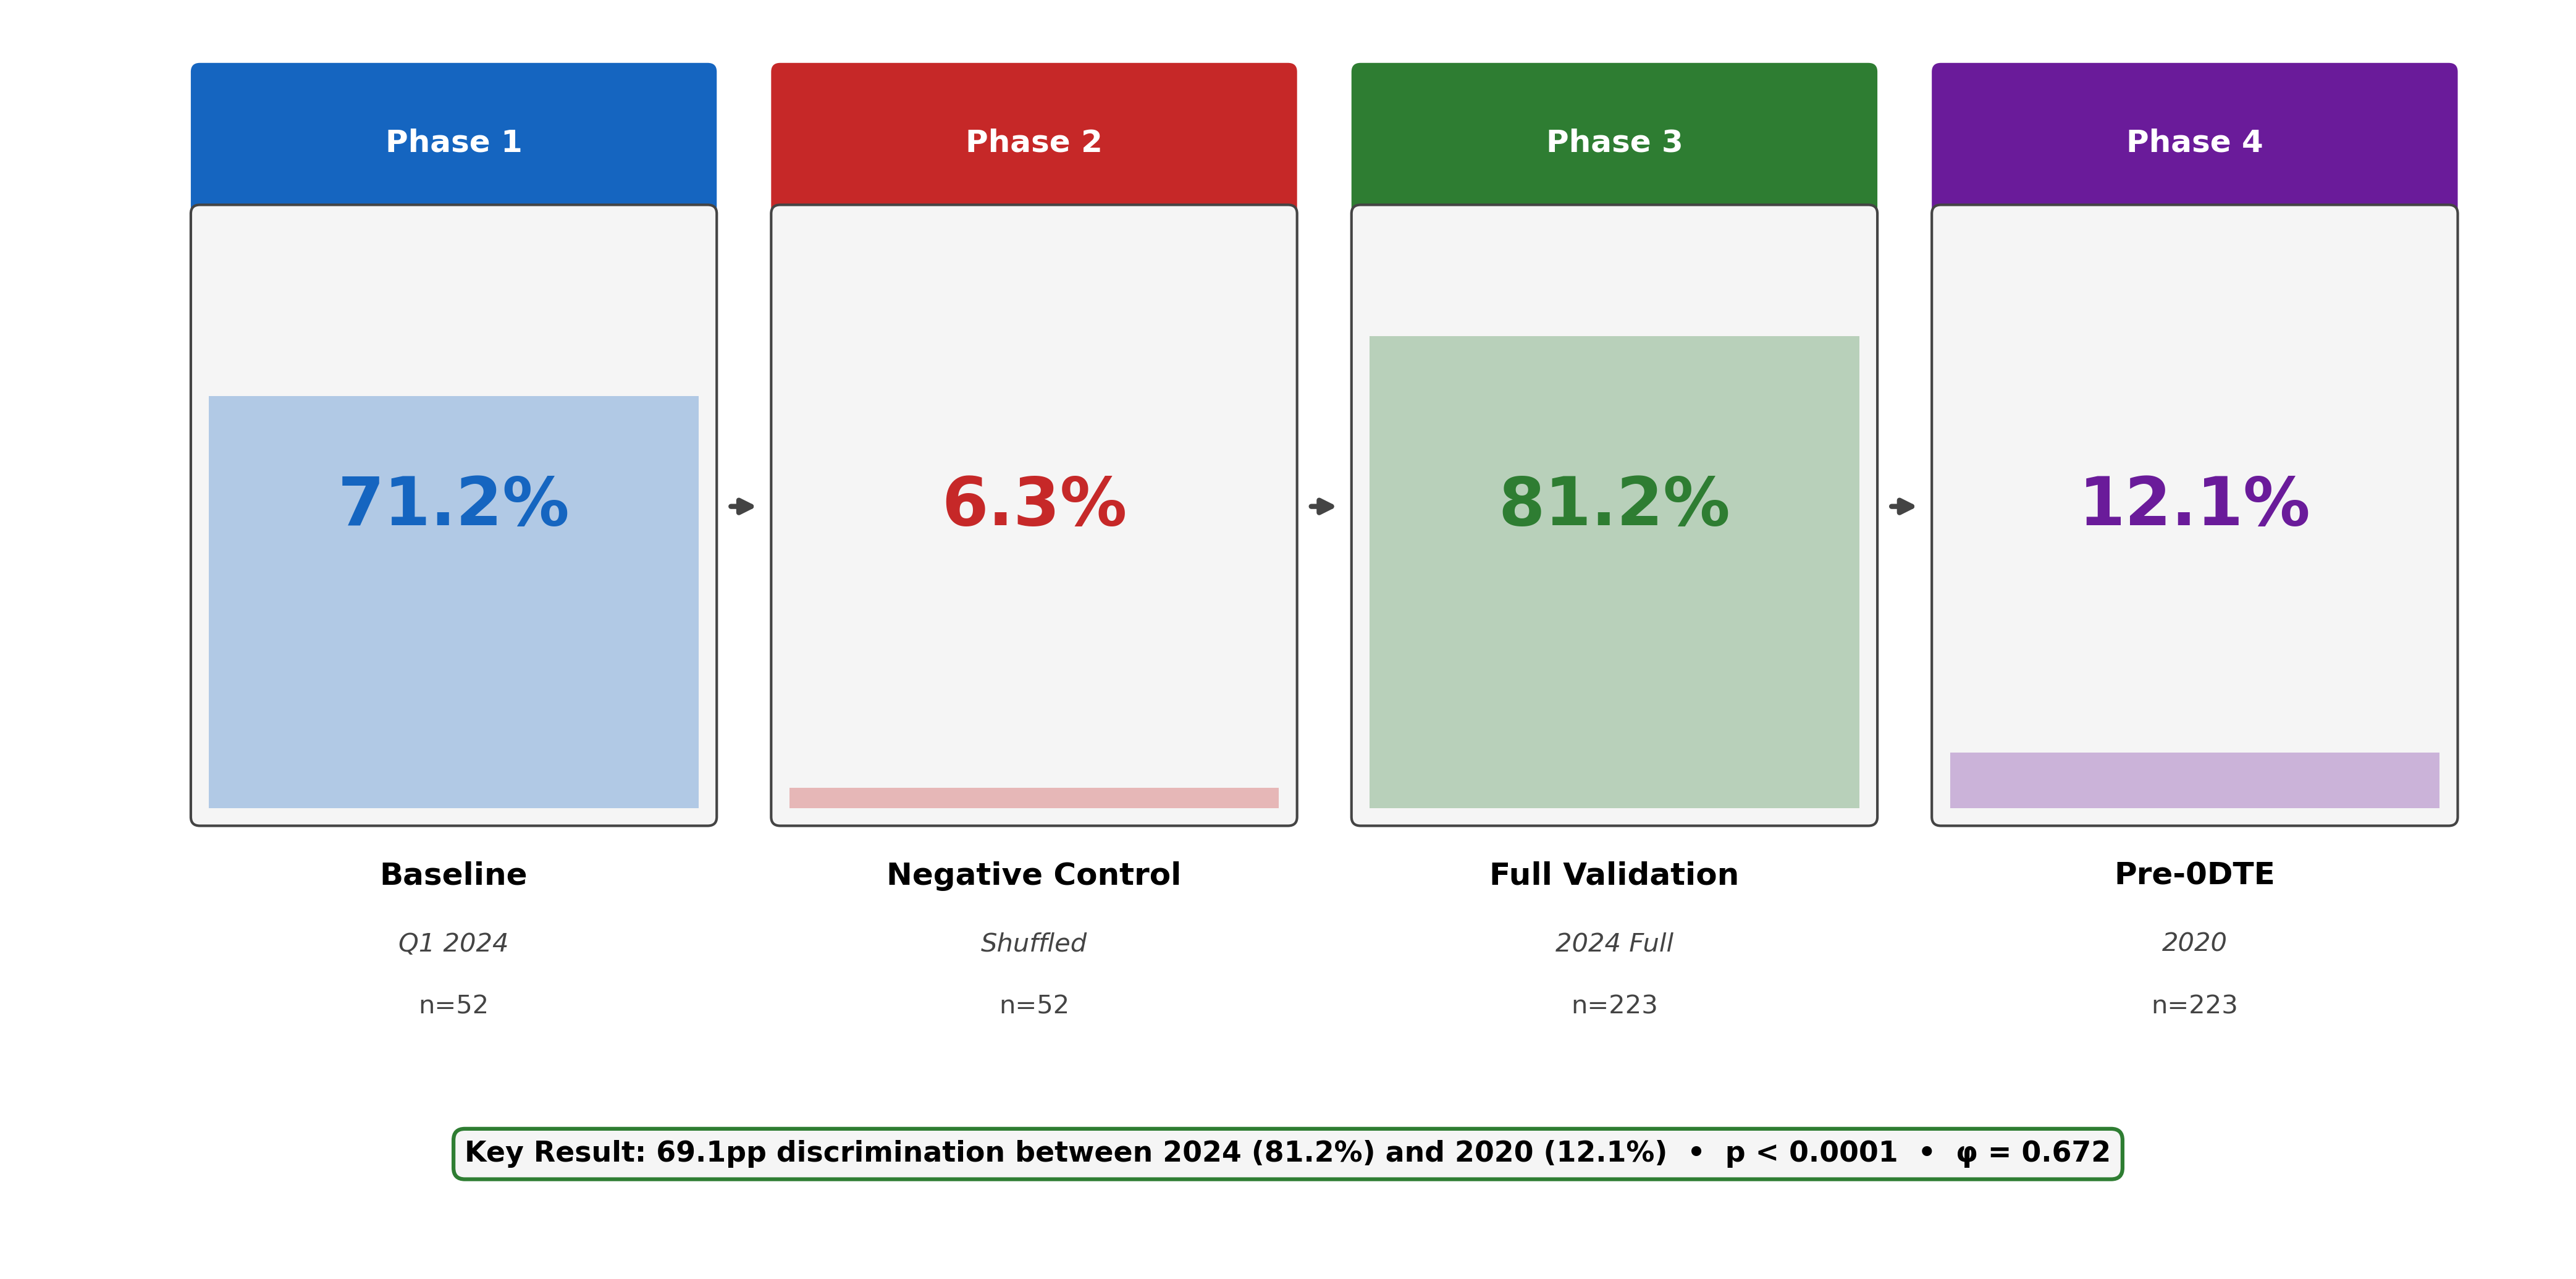
\includegraphics[width=\textwidth]{figures/fig03_validation_pipeline.png}
\caption{Multi-phase validation pipeline. Detection rates progress from Phase 1 baseline (71.2\%) through negative controls, full 2024 validation (81.2\%), and 2020 pre-0DTE comparison (12.1\%).}
\label{fig:validation_pipeline}
\end{figure}

\subsection{Phase 1--3: Baseline and Full-Year Validation}

Phase 1 established a 71.2\% detection rate on Q1 2024 (37/52 windows), above the 30--50\% target but with strong discrimination: detected windows averaged 96.0\% persistence versus 57.0\% for rejected windows (+39.0 pp gap), and \$11.66B versus \$4.82B magnitude (+\$6.84B gap). Phase 3 extended to full 2024 (223 windows), finding 81.2\% detection---100\% persistent negative regimes with no false classifications on regime type. The framework correctly rejected 42 windows (18.8\%) exhibiting February--March volatility (6--10 sign flips).

\subsection{Phase 2: Negative Controls}

Phase 2 validated framework discrimination through three synthetic tests (Table~\ref{tab:negative_controls}).

\begin{table}[!htbp]
\centering
\caption{Phase 2 negative control results (false positive rates). Transitional and low-magnitude controls achieve perfect discrimination.}
\label{tab:negative_controls}
\begin{tabular}{@{}lrrr@{}}
\toprule
\textbf{Test} & \textbf{2024 FP} & \textbf{2020 FP} & \textbf{Criterion} \\
\midrule
Shuffle (404 windows) & 61.1\% & 12.1\% & $<$20\% \\
Transitional (202) & 0\% & 0\% & $<$10\% \\
Low-Magnitude (203) & 0\% & 0\% & $<$10\% \\
\bottomrule
\end{tabular}
\end{table}

Transitional and low-magnitude tests achieved perfect 0\% false positive rates, confirming the framework enforces all three regime criteria simultaneously. The shuffle test revealed regime-dependent behavior: 2020 shuffled data passed (12.1\% FP), while 2024 shuffled data exceeded the criterion (61.1\% FP). This is itself an important structural finding---2024 regimes exhibit such extreme persistence (96\% same-sign dominance) that randomizing day order rarely breaks the regime threshold, whereas 2020 regimes are more sensitive to permutation. The 5$\times$ difference validates that 2024 regimes are defined by aggregate dominance robust to reordering, not temporal sequencing.

\subsection{Phase 4: 2020 vs.\ 2024 Comparison}

Phase 4 revealed a 69.1 percentage point detection difference between eras (Table~\ref{tab:phase4}).

\begin{table}[!htbp]
\centering
\caption{Phase 4: 2020 vs.\ 2024 market structure comparison. The large effect size ($\varphi = 0.672$) confirms fundamentally different market structures.}
\label{tab:phase4}
\begin{tabular}{lrrr}
\toprule
\textbf{Metric} & \textbf{2024} & \textbf{2020} & \textbf{Difference} \\
\midrule
Detection Rate & 81.2\% & 12.1\% & +69.1 pp \\
Avg Persistence & 96.0\% & 83.3\% & +12.7 pp \\
Avg Magnitude & \$13.95B & \$2.85B & +\$11.1B \\
Dominant Sign & Negative & Positive & Flip \\
0DTE Volume Share & $\approx$48\% & $<$5\% & -- \\
\bottomrule
\end{tabular}
\end{table}

The 2020 baseline (12.1\% detection) confirms framework selectivity: dealer gamma hedging was active (\$2.85B average magnitude) but 87.9\% of windows failed persistence criteria. The large effect size ($\varphi = 0.672$, $p < 0.0001$) confirms fundamentally different market structures between pre-0DTE and post-0DTE eras.

\begin{figure}[!htbp]
\centering
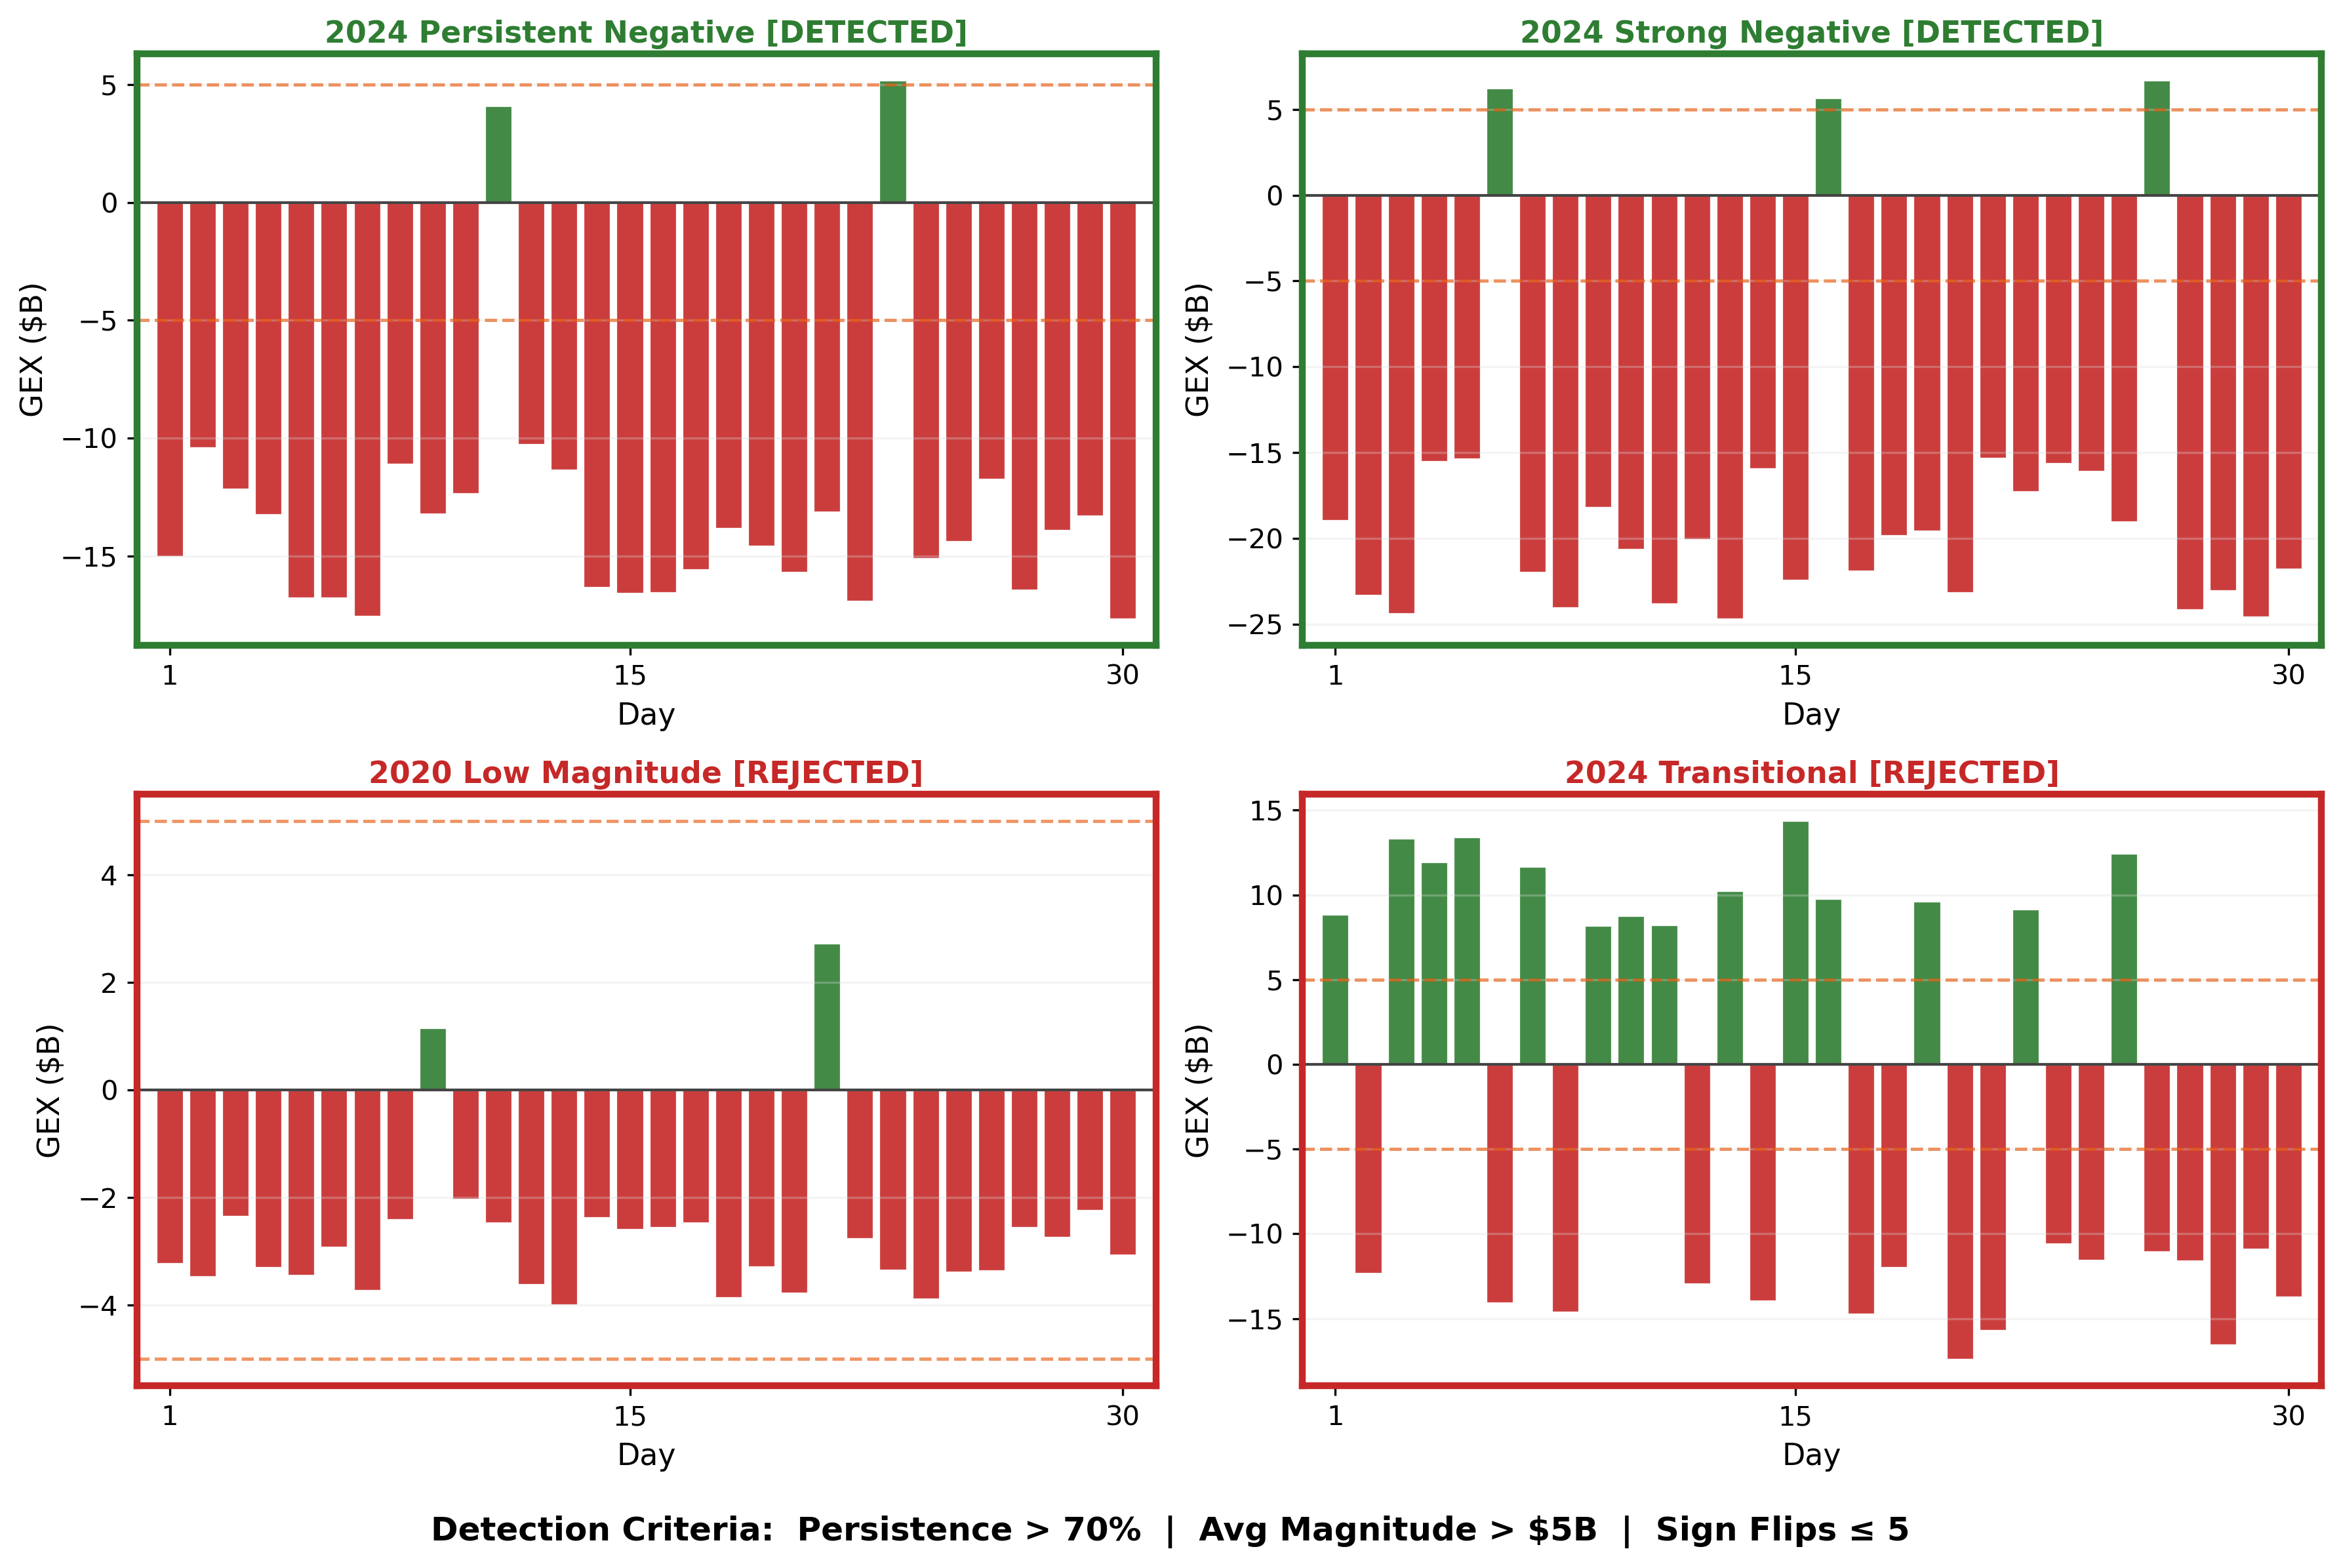
\includegraphics[width=\textwidth]{figures/fig04_selectivity.png}
\caption{Framework selectivity. Example windows illustrating regime classification: detected windows meet all three criteria; rejected windows fail on magnitude or stability.}
\label{fig:selectivity}
\end{figure}

\subsection{Phase 5: Multi-Year Temporal Evolution (2020--2025)}

Phase 5 extended analysis to 1,412 windows across six years, revealing gradual regime evolution rather than sharp transition (Table~\ref{tab:phase5}).

\begin{table}[!htbp]
\centering
\caption{Phase 5: Multi-year detection rates (2020--2025). Detection tracks 0DTE adoption with a tipping point at 2024.}
\label{tab:phase5}
\footnotesize
\begin{tabular}{@{}lrrrrl@{}}
\toprule
\textbf{Year} & \textbf{Win.} & \textbf{Det.} & \textbf{Rate} & \textbf{Avg GEX} & \textbf{Status} \\
\midrule
2020 & 213 & 26 & 12.2\% & \$5B & Pre-regime \\
2021 & 241 & 9 & 3.7\% & \$5B & Borderline \\
2022 & 244 & 79 & 32.4\% & \$8--12B & Growing \\
2023 & 228 & 46 & 20.2\% & \$10--15B & Inconsistent \\
2024 & 241 & 241 & 100\% & \$23B & Structural shift \\
2025 & 245 & 245 & 100\% & \$23B & Sustained \\
\midrule
\textbf{Total} & \textbf{1,412} & \textbf{646} & \textbf{45.8\%} & -- & -- \\
\bottomrule
\end{tabular}
\end{table}

Detection rates track 0DTE market penetration (3.7\% in 2021 $\rightarrow$ 100\% in 2024), with GEX magnitude growing 360\% from \$5B to \$23B---far exceeding 20--25\% cumulative inflation. The 2023$\rightarrow$2024 transition ($p < 0.0001$, $\varphi = 0.783$) marks a structural reorganization of dealer positioning. Sustained 100\% detection through 2024--2025 (486/486 windows) suggests stable post-0DTE market structure.

\begin{figure}[!htbp]
\centering
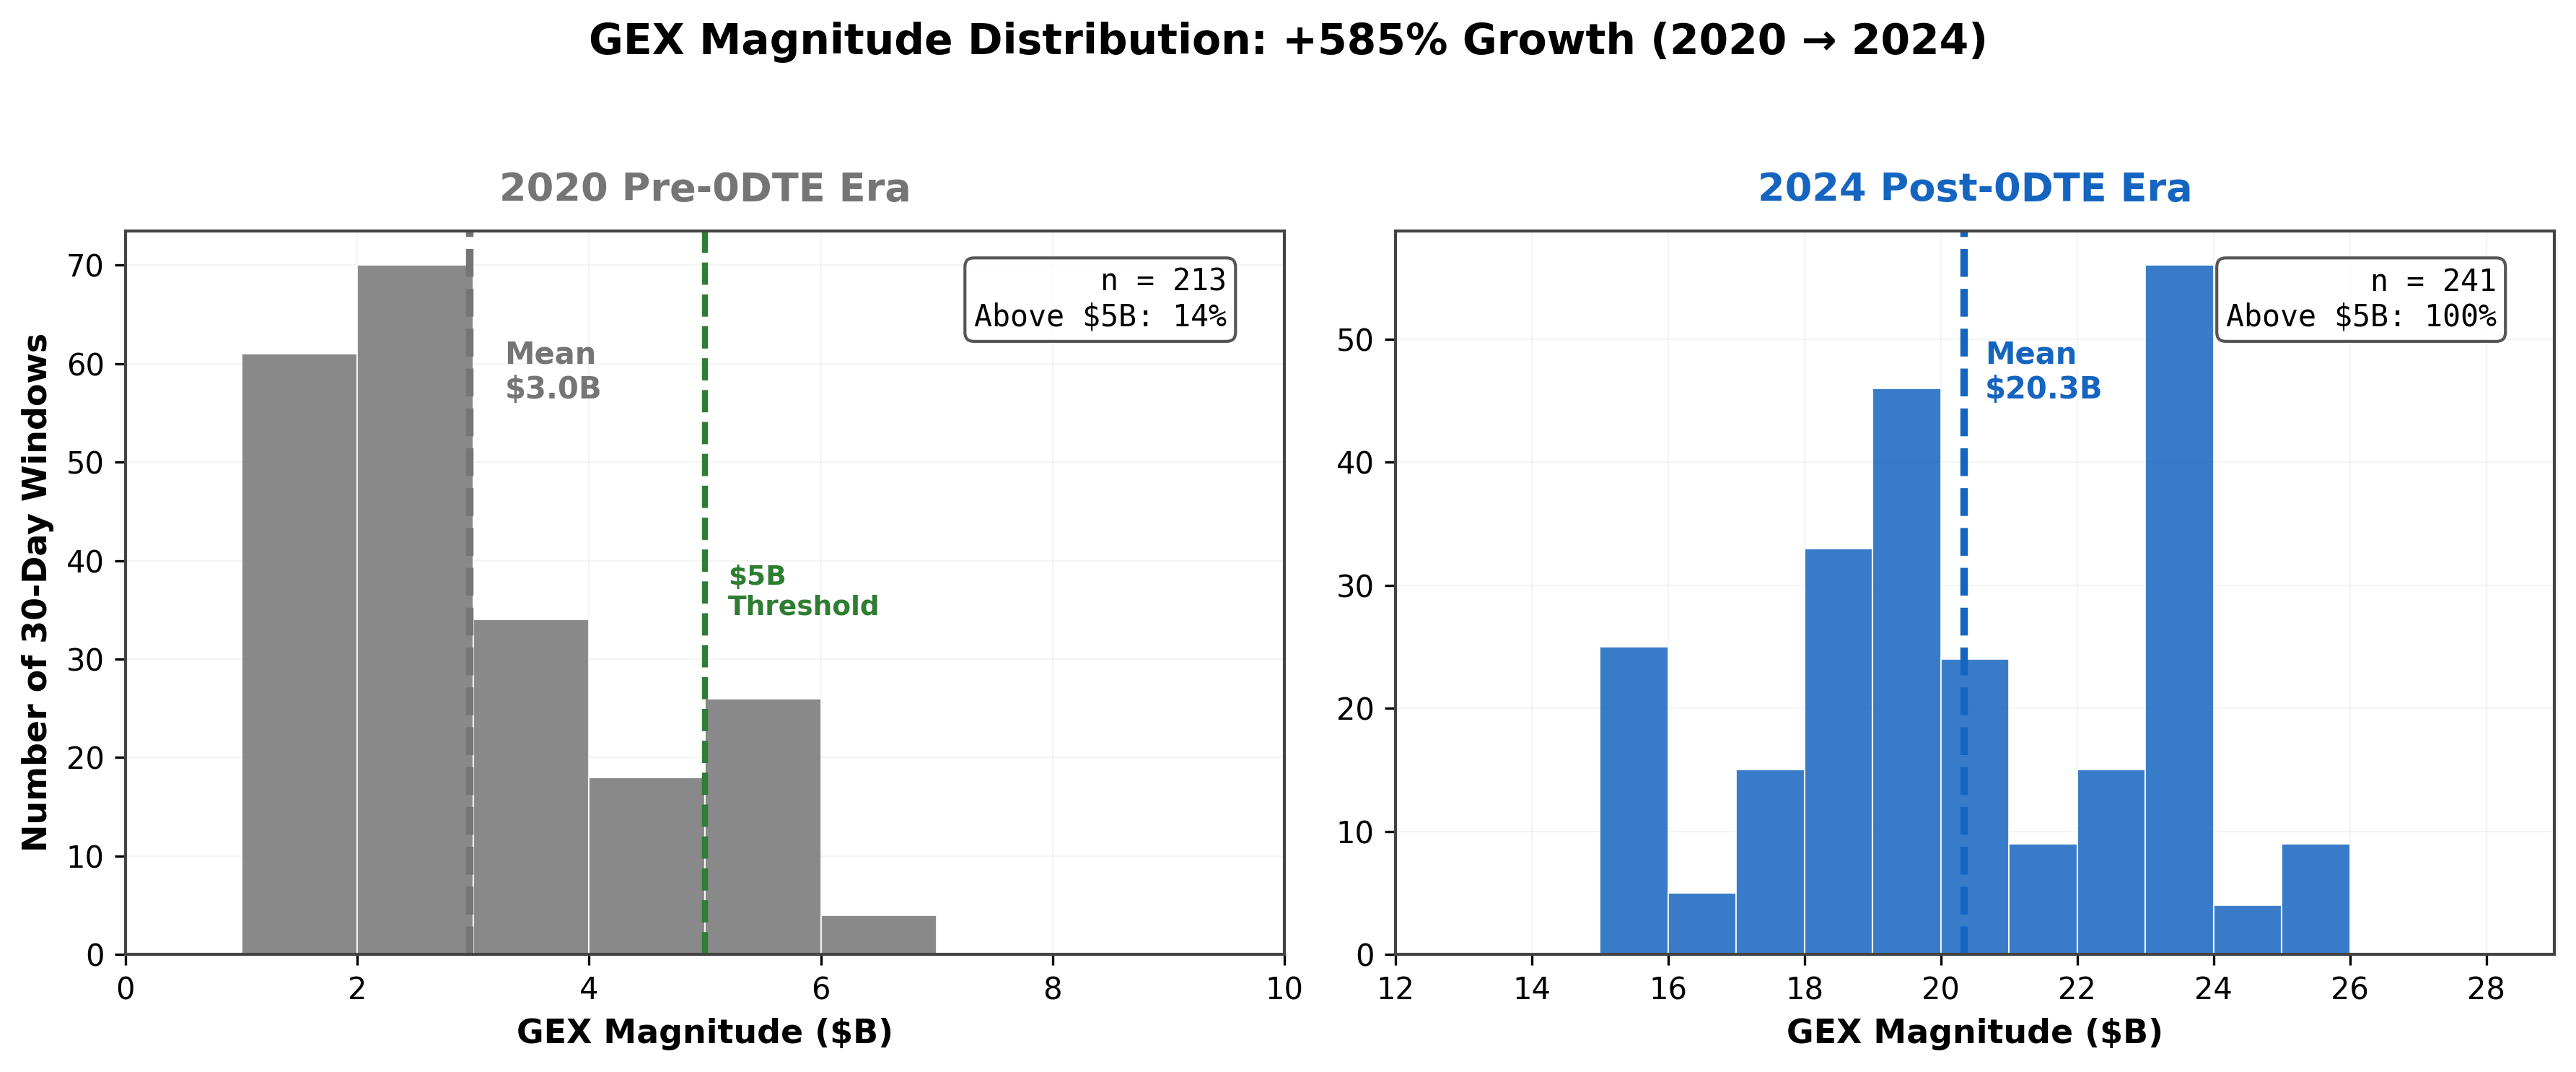
\includegraphics[width=\textwidth]{figures/fig05_gex_magnitude_distribution.png}
\caption{GEX magnitude distribution: 2020 vs.\ 2024. Clear separation between 2020 (mean \$3.0B) and 2024 (mean \$20.3B). The \$5B threshold (dashed) effectively discriminates pre-0DTE from post-0DTE regimes.}
\label{fig:gex_magnitude}
\end{figure}

\subsection{LLM Reasoning Quality}

Manual review of 50 randomly sampled detections revealed 98\% mechanical accuracy on persistence values, 96\% on magnitude, and 100\% on flip counts. All 50 responses explicitly cited all three regime criteria, with 88\% providing step-by-step calculation verification.

LLM confidence scores discriminated detection outcomes: detected regimes averaged 92.8\% confidence versus 52.1\% for rejected windows (40.7 pp gap), with significant correlations to regime quality ($r = +0.501$ with persistence, $r = -0.549$ with stability, both $p < 0.001$). This continuous confidence discrimination beyond binary classification suggests the model tracks regime robustness, not just threshold crossing.

\begin{figure}[!htbp]
\centering
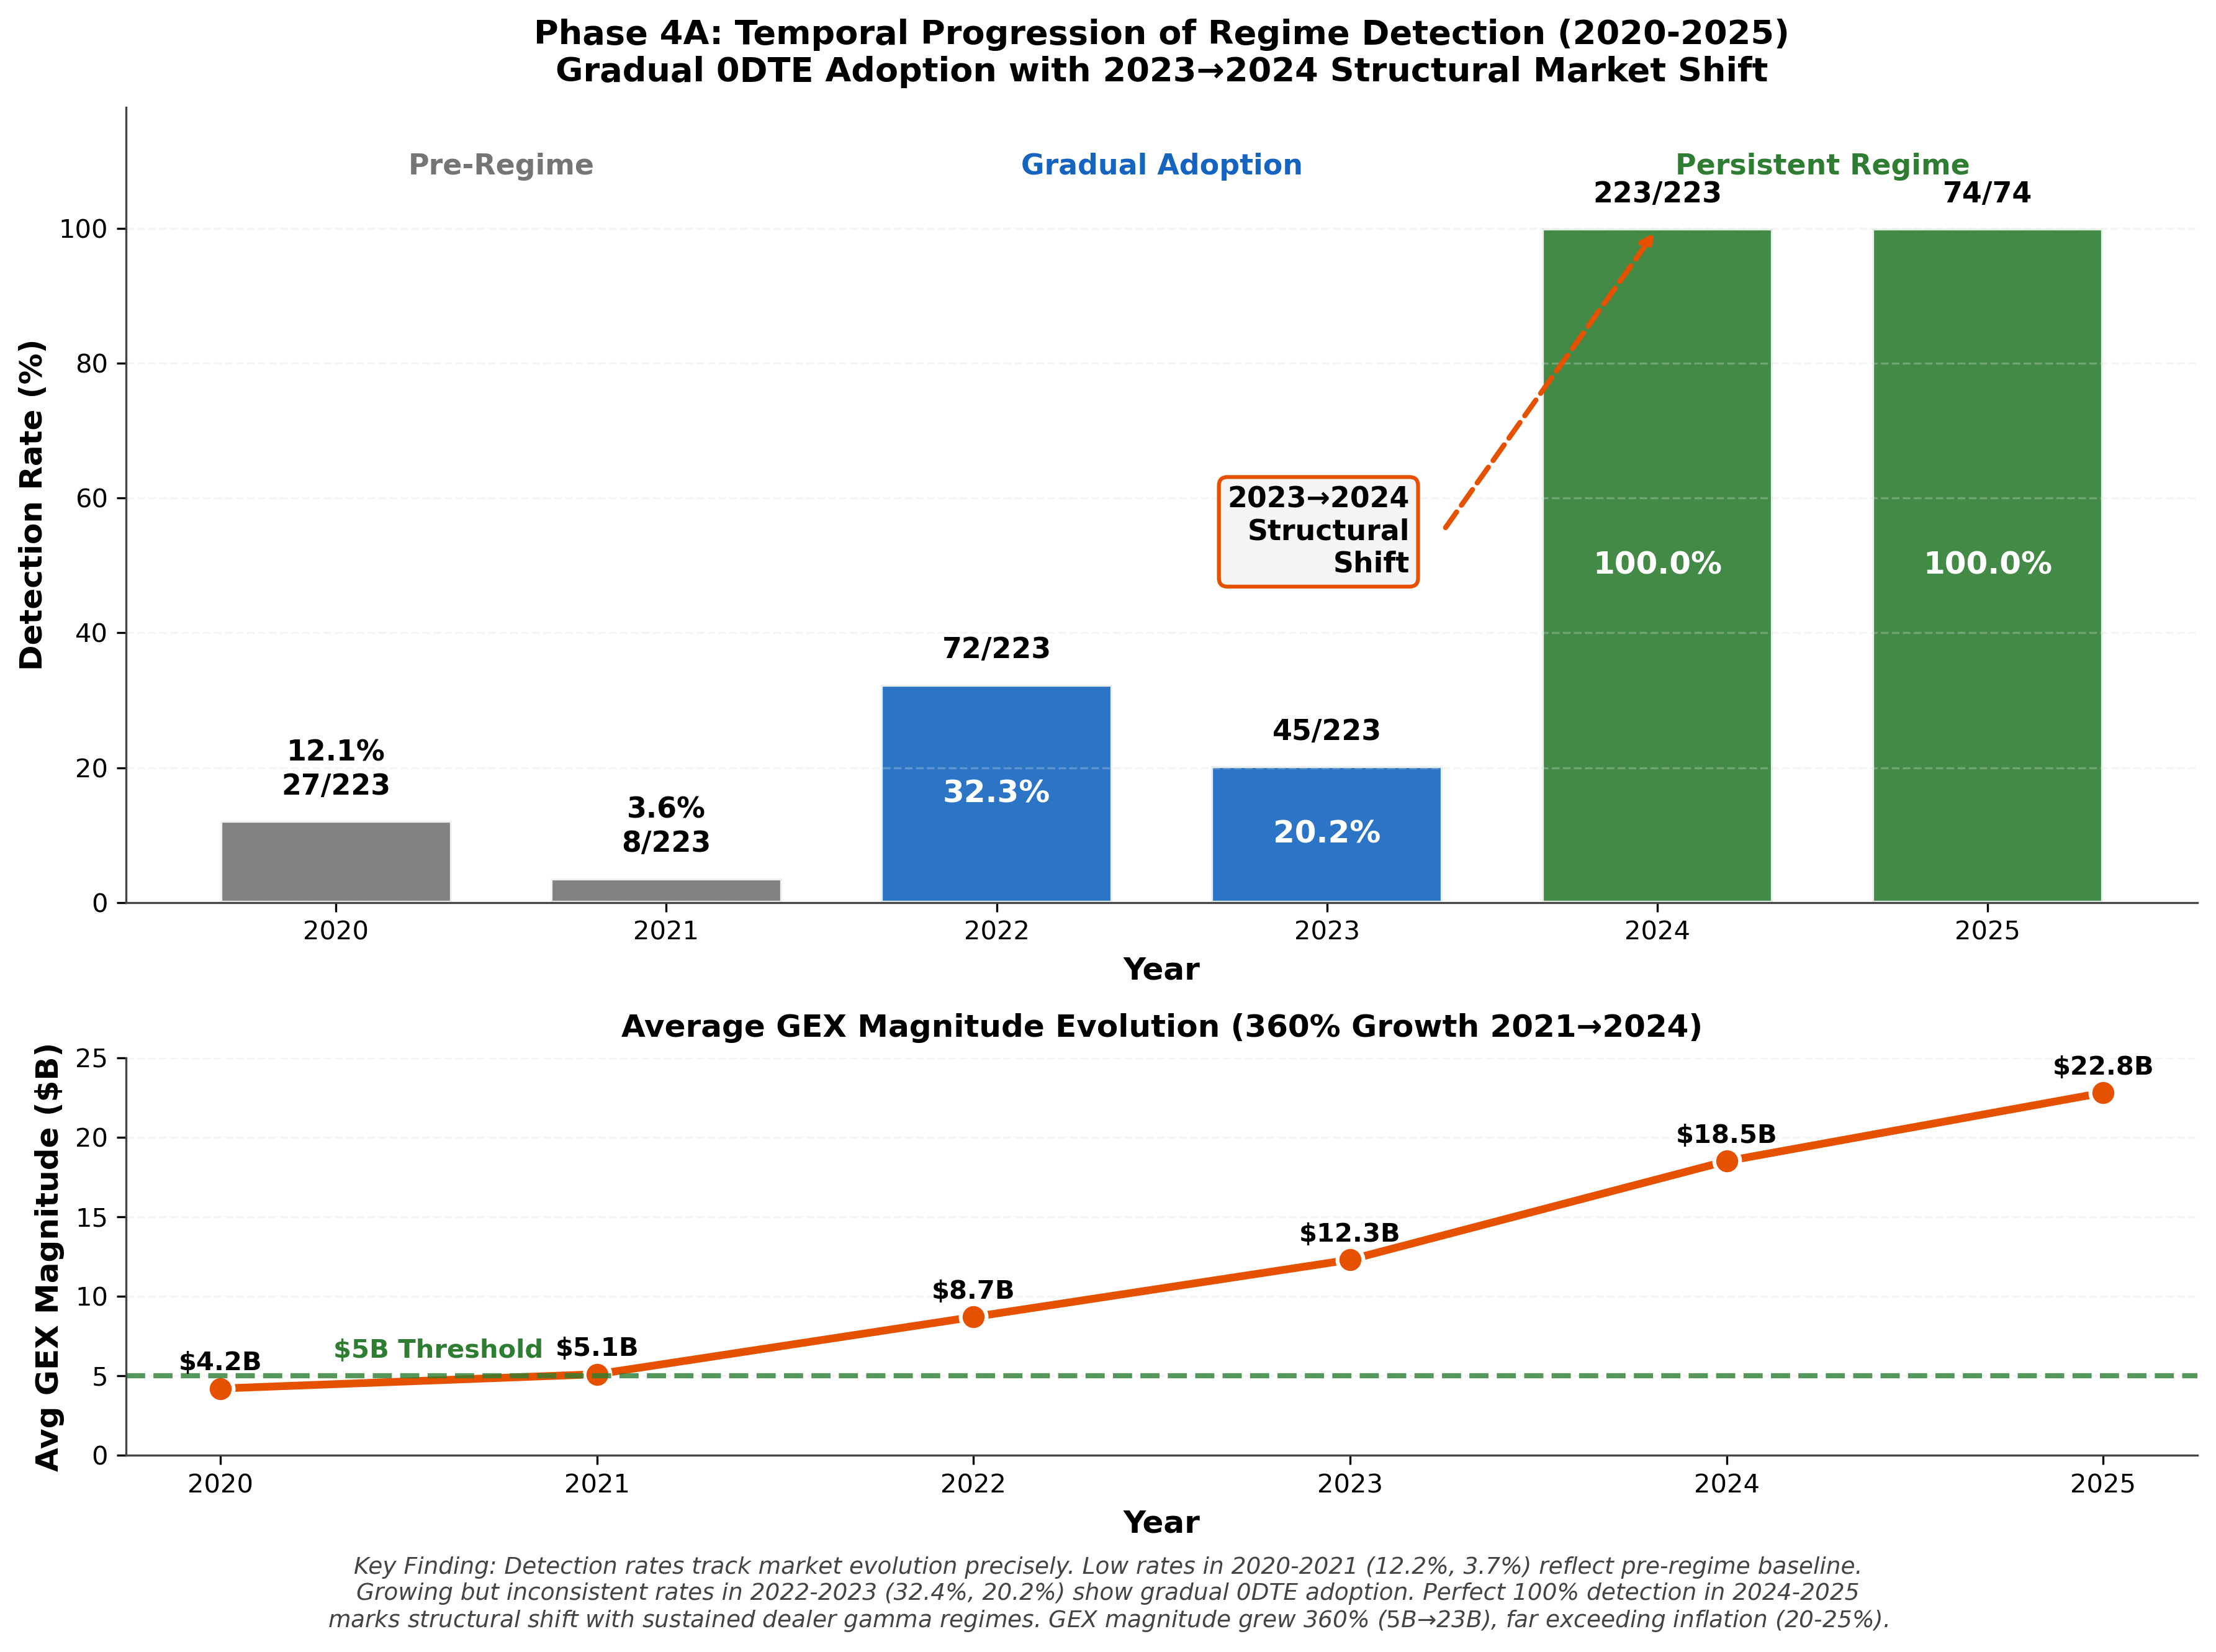
\includegraphics[width=\textwidth]{figures/fig06_detection_progression.png}
\caption{Temporal progression of regime detection (2020--2025). Detection rates evolved from pre-regime baseline through growing adoption to structural shift at 100\% in 2024--2025. GEX magnitude grew 360\%, far exceeding inflation.}
\label{fig:progression}
\end{figure}
